%!TEX root = edance.tex
%%%%%%%%%%%%%%%%
%   CHAPTER 9  %
%%%%%%%%%%%%%%%%
\chapter{MOS Transistor Small-Signal Models}
\label{ch:ch09_mos_ss_dc}
\graphicspath{{./figs_mos_ss_dc/}}
%%%%%%%%%%%%%%%%%%%%%%%%%%%%%%%%%%%%%%%%%%%%%%%%%%%%%%%%%%%%%%%%%%%%%%%%%%%%%%%%%%%%%%%%
%%%%%%%%%%%%%%%%%%%%%%%%%%%%%%%%%%%%%%%%%%%%%%%%%%%%%%%%%%%%%%%%%%%%%%%%%%%%%%%%%%%%%%%%
%                                   SECTION 9.1                                        %
%%%%%%%%%%%%%%%%%%%%%%%%%%%%%%%%%%%%%%%%%%%%%%%%%%%%%%%%%%%%%%%%%%%%%%%%%%%%%%%%%%%%%%%%
%%%%%%%%%%%%%%%%%%%%%%%%%%%%%%%%%%%%%%%%%%%%%%%%%%%%%%%%%%%%%%%%%%%%%%%%%%%%%%%%%%%%%%%%
\section{Chapter Preview}
When the inventors of the bipolar transistor at Bell Labs first built a working device (see \emph{Fig.~\ref{fig:bjt_invent}}), the next thing they did was to build an audio amplifier to prove that the transistor was actually working.  In this chapter we are going to introduce you to your first amplifier, and discuss how we go about analyzing the amplifier using the $I$-$V$ equations we derived in the previous chapter.  The amplifier will be a \emph{"common source"} amplifier.  We will discuss bias points, also known as the operating point, and what happens when a signal is applied.  Throughout the chapter we will make a very common and important assumption, which leads to the \emph{Small Signal Analysis} technique.  This technique simply states that if the signal amplitudes are small (we will define what "small" means), we can analyze the circuit using linear techniques. This leads us to a linearized model of the circuit, which is much easier to analyze.  Finally, we will introduce the equivalent linear circuit model for a MOS transistor, and derive its small-signal parameters, such as transconductance and output resistance.  In the next chapter, we will cover charge storage effects and modify the model to include capacitors, which are needed to properly account for the frequency response of amplifiers.
%%%%%%%%%%%%%%%%%%%%%%%%%%%%%%%%%%%%%%%%%%%%
%                 FIGURE                   %
%%%%%%%%%%%%%%%%%%%%%%%%%%%%%%%%%%%%%%%%%%%%
\begin{figure}[tb]
\centering
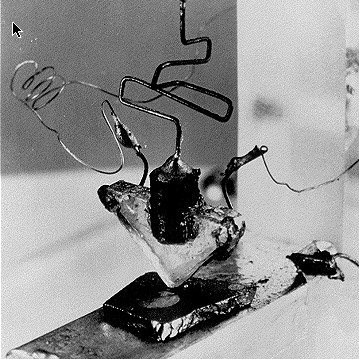
\includegraphics[width=.5\columnwidth]{bjt_invent.png}
\caption{The first transistor amplifier was demonstrated on December 23, 1947, by three scientist at Bell Laboratories.  The three scientists were Dr. Shockley, Dr. Bardeen, and Dr. Brattain, honored with the Nobel Prize in 1956.}
\label{fig:bjt_invent}
\end{figure}
%%%%%%%%%%%%%%%%%%%%%%%%%%%%%%%%%%%%%%%%%%%%%%%%%%%%%%%%%%%%%%%%%%%%%%%%%%%%%%%%%%%%%%%%
%%%%%%%%%%%%%%%%%%%%%%%%%%%%%%%%%%%%%%%%%%%%%%%%%%%%%%%%%%%%%%%%%%%%%%%%%%%%%%%%%%%%%%%%
%                                   SECTION 9.2                                        %
%%%%%%%%%%%%%%%%%%%%%%%%%%%%%%%%%%%%%%%%%%%%%%%%%%%%%%%%%%%%%%%%%%%%%%%%%%%%%%%%%%%%%%%%
%%%%%%%%%%%%%%%%%%%%%%%%%%%%%%%%%%%%%%%%%%%%%%%%%%%%%%%%%%%%%%%%%%%%%%%%%%%%%%%%%%%%%%%%
\section{Introduction to Amplifiers}
%%%%%%%%%%%%%%%%%%%%%%%%%%%%%%%%%%%%%%%%%%%%
%             SUBSECTION 9.2.1             %
%%%%%%%%%%%%%%%%%%%%%%%%%%%%%%%%%%%%%%%%%%%%
\subsection{A Simple Circuit: A MOS Amplifier}
%%%%%%%%%%%%%%%%%%%%%%%%%%%%%%%%%%%%%%%%%%%%
%                 FIGURE                   %
%%%%%%%%%%%%%%%%%%%%%%%%%%%%%%%%%%%%%%%%%%%%
\begin{figure}[tb]
\centering
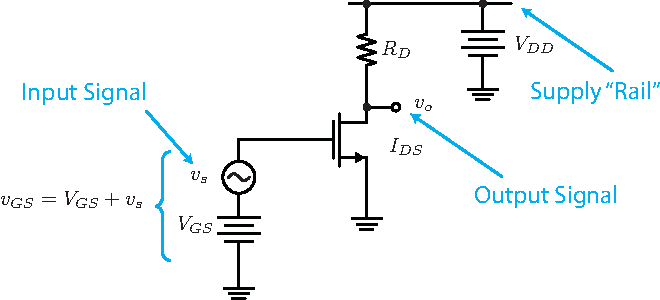
\includegraphics[width=.75\columnwidth]{csamp_signals}
\caption{A common source transistor amplifier biased with DC voltages $V_{GS}$ and $V_{DD}$ and driven by an AC signal $v_s$ at the input.  The output signal is taken at the drain side.}
\label{fig:csamp_signals}
\end{figure}
%%%%%%%%%%%%%%%%%%%%%%%%%%%%%%%%%%%%%%%%%%%%
A MOS amplifier is shown in \emph{Fig.~\ref{fig:csamp_signals}}.  Notice that a MOS transistor sits at the core of the amplifier.  The input signal is applied to the gate, and the output is taken at the drain of the transistor.  The source is ground (and so is the body, even though it's not shown explicitly).  MOS devices are biased in the saturation region so that the output current is only a function of the gate-source voltage (approximately), which means the transistor is acting like a voltage-controlled current source (see \emph{Fig.~\ref{fig:mos_building_block}}).  In order to turn the MOS "on" and bias it in saturation, the drain is pulled up through a resistor\footnote{See Appendix ~\ref{app:networks} for an explanation of pull-up and pull-down networks.} $R_D$, which is connected to the supply.  The "on" current $I_{DS,sat}$ and the resistor $R_D$ are selected together to determine the operating point.  On the gate side the appropriate $V_{GS}$ needs to be supplied to obtain the desired current $I_{DS,sat}$.  The input signal $v_{s}$ is applied in series with this gate bias voltage $V_{GS}$.
%%%%%%%%%%%%%%%%%%%%%%%%%%%%%%%%%%%%%%%%%%%%
%                 FIGURE                   %
%%%%%%%%%%%%%%%%%%%%%%%%%%%%%%%%%%%%%%%%%%%%
\begin{figure}[tb]
\centering
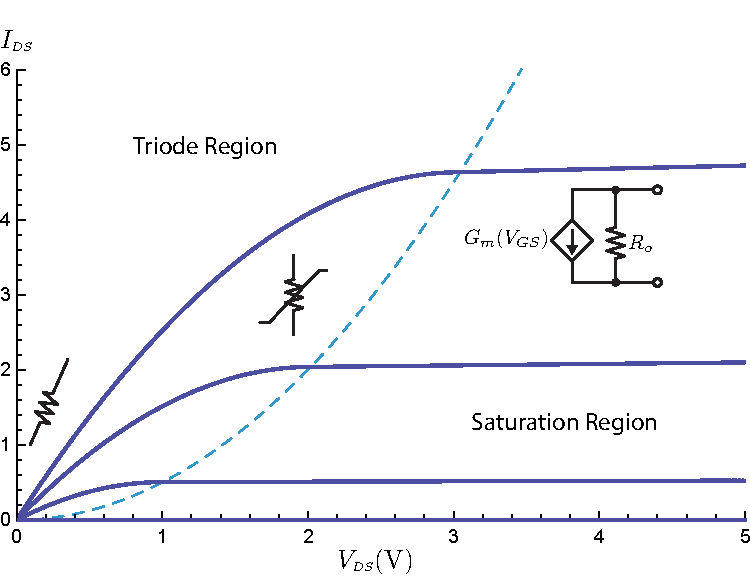
\includegraphics[width=.75\columnwidth]{mos_building_block}
\caption{The MOS $I_{DS}$ vs $V_{DS}$ family of curves in saturation are nearly flat, indicating that the gate is largely responsible for the current.  The device acts like a controlled current source (amplifier).}
\label{fig:mos_building_block}
\end{figure}
%%%%%%%%%%%%%%%%%%%%%%%%%%%%%%%%%%%%%%%%%%%%
A plot of input and output signals is shown in \emph{Fig.~\ref{fig:gain}}.  Note that the DC value is subtracted out.  In many cases the DC value is not of interest.  A good example is an audio amplifier.  The speaker only responds to AC signals, and sound is an AC signal.  The important point about this plot is the voltage excursions at the output are much larger than the input, providing voltage gain.  As shown in \emph{Fig.~\ref{fig:id_vgs_slope}}, the key insight is that a gate voltage modulates the source-drain current, and this current can produce a much larger drain-source voltage.  This is because the drain-source current only depends on the value of the gate voltage, and not so much on the drain-source voltage, in the saturation region. The goal of this chapter is to derive this plot in a step-by-step fashion.
%%%%%%%%%%%%%%%%%%%%%%%%%%%%%%%%%%%%%%%%%%%%
%                 FIGURE                   %
%%%%%%%%%%%%%%%%%%%%%%%%%%%%%%%%%%%%%%%%%%%%
\begin{figure}[tb]
\centering
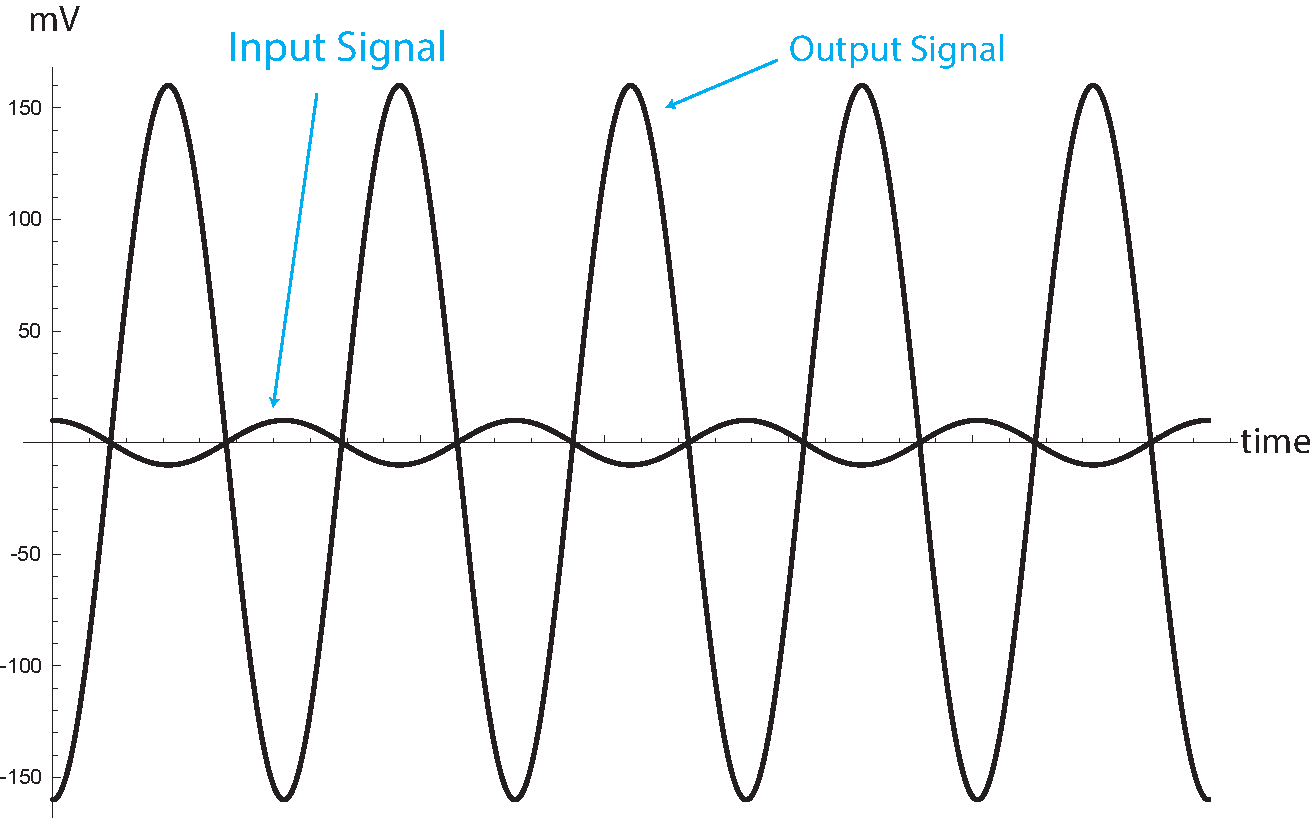
\includegraphics[width=.75\columnwidth]{gain}
\caption{The input signal $v_s$ and output signal $v_o$ plotted versus time.  The output voltage is an amplified (and inverted) copy of the input.}
\label{fig:gain}
\end{figure}
%%%%%%%%%%%%%%%%%%%%%%%%%%%%%%%%%%%%%%%%%%%%
%                 FIGURE                   %
%%%%%%%%%%%%%%%%%%%%%%%%%%%%%%%%%%%%%%%%%%%%
\begin{figure}[tb]
\centering
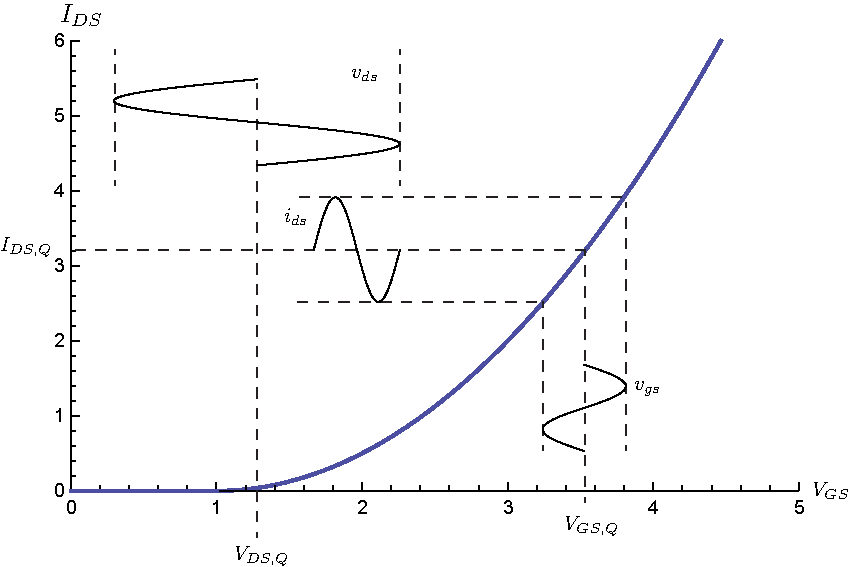
\includegraphics[width=.75\columnwidth]{ids_vgs_vds}
\caption{To illustrate the transconductance of a MOSFET, we bias the device at a particular operation or Q point and excite it with a small-signal AC around the operating point.  The resulting output current can produce a larger drain voltage by using a large load resistor.}
\label{fig:ids_vgs_vds}
\end{figure}
%%%%%%%%%%%%%%%%%%%%%%%%%%%%%%%%%%%%%%%%%%%%
%             SUBSECTION 9.2.2             %
%%%%%%%%%%%%%%%%%%%%%%%%%%%%%%%%%%%%%%%%%%%%
\subsection{Common-Source Amplifier}
The amplifier that we have presented is known as a \textbf{Common Source}\index{Amplifers!Common source} (CS) amplifier, because the transistor source terminal is in common with both the input signal and the output signal.  Or more simply, the source is grounded to the "common" node, also known as the reference voltage.  Another way to understand this is that the "common" node does not carry the signal (both input and output).  Since a transistor has three terminals (actually 4, but the body is usually tied to the source), and a voltage is defined by 2 terminals, then you can readily count and see that there are three simple configurations for a single transistor amplifier, "common source", "common drain", and "common gate".  In this chapter we'll focus on the common source variety.
%%%%%%%%%%%%%%%%%%%%%%%%%%%%%%%%%%%%%%%%%%%%%%%%%%%%%%%%%%%%%%%%%%%%%%%%%%%%%%%%%%%%%%%%
%%%%%%%%%%%%%%%%%%%%%%%%%%%%%%%%%%%%%%%%%%%%%%%%%%%%%%%%%%%%%%%%%%%%%%%%%%%%%%%%%%%%%%%%
%                                   SECTION 9.3                                        %
%%%%%%%%%%%%%%%%%%%%%%%%%%%%%%%%%%%%%%%%%%%%%%%%%%%%%%%%%%%%%%%%%%%%%%%%%%%%%%%%%%%%%%%%
%%%%%%%%%%%%%%%%%%%%%%%%%%%%%%%%%%%%%%%%%%%%%%%%%%%%%%%%%%%%%%%%%%%%%%%%%%%%%%%%%%%%%%%%
\section{Operating Points}
%%%%%%%%%%%%%%%%%%%%%%%%%%%%%%%%%%%%%%%%%%%%
%                 FIGURE                   %
%%%%%%%%%%%%%%%%%%%%%%%%%%%%%%%%%%%%%%%%%%%%
\begin{figure}[tb]
\centering
\subcaptionbox{(a) \label{fig:csamp_oppoint} }{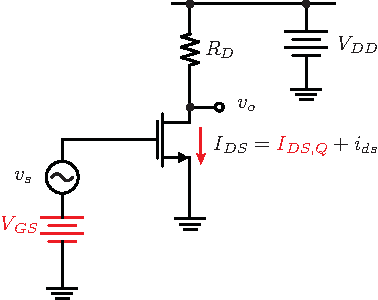
\includegraphics[scale=1]{csamp_oppoint}}
\subcaptionbox{(b) \label{fig:csamp_dc}}{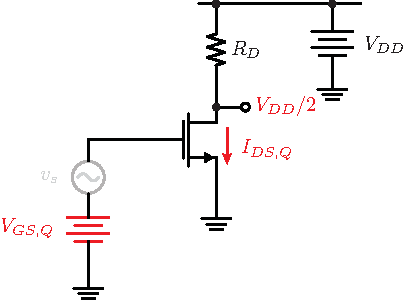
\includegraphics[scale=1]{csamp_dc}}
\caption{MOS amplifier (a) DC setup.  The voltage source $V_{GS}$ determines the quiescent current $I_{DS,Q}$, which in turn determines the output (b) DC operating voltage.  Notice the DC operating point is independent of the AC input signals.} 
\end{figure}
%%%%%%%%%%%%%%%%%%%%%%%%%%%%%%%%%%%%%%%%%%%%
The bias voltages (DC voltages shown in red in \emph{Fig.~\ref{fig:csamp_oppoint}}) that you apply to the MOSFET determine its \textbf{operating point}\index{Operating point}, also known as the \textbf{quiescent point}\index{Quiescent point}, or \textbf{Q-point} for simplicity.  How you bias the MOSFET will make a big difference in how it functions.  If we operate with a sufficiently high $V_{GS}$ \emph{and} a sufficiently high $V_{DS}$ to place the device in the saturation region, we can make a very good amplifier.
%%%%%%%%%%%%%%%%%%%%%%%%%%%%%%%%%%%%%%%%%%%%
%             SUBSECTION 9.3.1             %
%%%%%%%%%%%%%%%%%%%%%%%%%%%%%%%%%%%%%%%%%%%%
\subsection{Small Signal vs. Large Signal}
We derived that $I_{DS}$ vs. $V_{GS}$ is a quadratic function for $V_{GS} > V_T$.  Therefore large changes in $V_{GS}$ result in quadratically larger changes at the output.  However, small changes in $V_{GS}$ (denoted as $v_{gs}$) will produce linear changes at the output.  We can show this using a Taylor series\footnote{See Appendix ~\ref{app:calc} for a review of the Taylor series} expansion:
    \begin{equation}
        {I_{DS}(V_{GS} + v_{gs})} \approx I_{DS} {(V_{GS})} + \frac{dI_{DS}}{dV_{GS}} \cdot v_{gs}  
    \end{equation}
In many applications of interest, we can make this approximation and assume the signals are small with respect to the bias points\index{Bias point}, which allows us to convert MOS transistor equations into linear equations, which are much simpler to analyze.
%%%%%%%%%%%%%%%%%%%%%%%%%%%%%%%%%%%%%%%%%%%%
%             SUBSECTION 9.3.2             %
%%%%%%%%%%%%%%%%%%%%%%%%%%%%%%%%%%%%%%%%%%%%
\subsection{Selecting the Output Bias Point}
As shown in \emph{Fig.~\ref{fig:csamp_dc}}, we must select the CS amplifier Q points to produce the desired response.  A common choice is to bias $V_{GS}$ so that the output is mid-rail (between $V_{DD}$ and ground).  This is a design choice, not a requirement, but doing so results in a large swing at the output.  Notice that the output cannot go larger than $V_{DD}$, and to provide gain (remain in saturation) it should not go lower than $V_{GS}-V_T$, so any drain-source voltage greater than $V_{DS,sat} = V_{GS}-V_T$ and smaller than $V_{DD}$ is possible.  Mid-rail is a good back-of-the-envelope value to maximize the AC sinusoidal swing (this assumes $V_{DS,sat}$ is very small).  This places a constraint on the DC drain current through the resistor:
    \begin{equation}
        {I_R} = \frac{{{V_{DD}} - {V_o}}}{{{R_D}}} = \frac{{{V_{DD}} - {V_{DS}}}}{{{R_D}}}
    \end{equation}
The resistor current flows into transistor:
    \begin{equation}
        {I_R} = {I_{DS,sat}}
    \end{equation}
We must ensure that this gives a self-consistent solution (transistor is biased in saturation)
    \begin{equation}
        {V_{DS}} > V_{DS,sat} = {V_{GS}} - {V_T}
    \end{equation}
%%%%%%%%%%%%%%%%%%%%%%%%%%%%%%%%%%%%%%%%%%%%
%             SUBSECTION 9.3.3             %
%%%%%%%%%%%%%%%%%%%%%%%%%%%%%%%%%%%%%%%%%%%%
\subsection{Finding the Input Bias Voltage}
For now let's ignore the output resistance (the term involving $\lambda$) to simplify the analysis:
    \begin{equation}
        {I_{DS,sat}} = \frac{W}{L}{\mu _n}{C_{ox}}\frac{1}{2}{({V_{GS}} - {V_{Tn}})^2}
    \end{equation}
This means that the current through the resistor is given by
    \begin{equation}
        {I_{{R_D}}} = \frac{{{V_{DD}}}}{{2{R_D}}} = {I_{DS,sat}} = \frac{W}{L}{\mu _n}{C_{ox}}\frac{1}{2}{({V_{GS}} - {V_{Tn}})^2}
    \end{equation}
Note that we assume the voltage drop across the resistor is $V_{DD}/2$, which was our design choice.  To make this a bit less abstract, let's use some typical numbers for a long channel transistor: $W=40\mu$m, $L = 2\mu$m,  $R_D = 25$k$\Omega$, $\mu_nCox = 100\mu$A/V$^2$, $V_T = 1$V, and $V_{DD} = 5$V.  Substituting numerical values:
    \begin{equation}
        \frac{{5{\rm{V}}}}{{50{\rm{k}}\Omega }} = 100{\rm{\mu A}} = 20 \cdot 100\frac{{{\rm{\mu A}}}}{{{{\rm{V}}^2}}} \cdot \frac{1}{2}{({V_{GS}} - 1)^2}
    \end{equation}
and solving for $V_{GS}$, we have $.1\mathrm{V} = {({V_{GS}} - 1V)^2}$, which gives ${V_{GS}} = 1.32$V.  %%%%%%%%%%%%%%%%%%%%%%%%%%%%%%%%%%%%%%%%%%%%
Let's make sure that our assumption of operating point was correct, namely that the device is in saturation.  The $V_{DS,sat}$ is given by ${V_{GS}} - {V_T} = .32$V, and by design $V_{DS} = 2.5$V, so $V_{DS,sat} < {V_{DS}} = 2.5$V, which confirms our assumption.
%%%%%%%%%%%%%%%%%%%%%%%%%%%%%%%%%%%%%%%%%%%%
%             SUBSECTION 9.3.4             %
%%%%%%%%%%%%%%%%%%%%%%%%%%%%%%%%%%%%%%%%%%%%
\subsection{Applying the AC Voltage:  The "Hard Way"}
To find the output signal, we'll take two approaches.  The first is the "hard way" because it involves many steps and a lot of approximations.  Later we'll introduce the "easy way" which leads directly to a linear circuit that we can analyze with known techniques.  
%%%%%%%%%%%%%%%%%%%%%%%%%%%%%%%%%%%%%%%%%%%%
In our first approach to solving for the output voltage, we will just use $v_{gs}$ in the equations for the total drain current $I_{DS}$  and find $v_o$ :
    \begin{equation}
        {V_{GS}} = {V_{GS,Q}} + {v_{gs}}
    \end{equation}
    \begin{equation}
        v_{gs} = {\hat V_s}\cos \omega t
    \end{equation}
    \begin{equation}
        {V_o} = {V_{DD}} - {R_D}{I_{DS}} = {V_{DD}} - {R_D}{\mu _n}{C_{ox}}\frac{W}{L}\frac{1}{2}{({V_{GS,Q}} + {v_{gs}} - {V_T})^2}
    \end{equation}
We are neglecting charge storage effects and we're ignoring the device output resistance to keep things simple.  Now let's solve for the output voltage $v_o$:
    \begin{equation}
        {V_o} = {V_{DD}} - {R_D}{I_{DS}} = {V_{DD}} - {R_D}\left( {\mu _n}{C_{ox}}\frac{W}{L}\frac{1}{2}{({V_{GS}} + {v_{gs}} - {V_T})^2} \right)
    \end{equation}
Focusing on the drain current, we note that it can be factored into two terms, the bias point $I_{DS,Q}$ and the signal:
    \begin{equation}
        I_{DS} = \underbrace{{\mu _n}{C_{ox}}\frac{W}{L}\frac{1}{2}{({V_{GS}} - {V_T})^2}}_{I_{DS,Q}}{\left( {1 + \frac{{{v_{gs}}}}{{{V_{GS}} - {V_T}}}} \right)^2}
    \end{equation}
The bias current $I_{DS,Q}$ was selected to produce a mid-rail output voltage:
    \begin{equation}
        {V_o} = {V_{DD}} - \underbrace{ {R_D}{I_{DS,Q}}}_{\frac{V_{DD}}{2}}{\left( {1 + \frac{{{v_{gs}}}}{{{V_{GS}} - {V_T}}}} \right)^2}
    \end{equation}
The above equation is the "Large Signal" output voltage as a function of the input voltage.
%%%%%%%%%%%%%%%%%%%%%%%%%%%%%%%%%%%%%%%%%%%%
%             SUBSECTION 9.3.5             %
%%%%%%%%%%%%%%%%%%%%%%%%%%%%%%%%%%%%%%%%%%%%
\subsection{Small-Signal Simplifications}
We linearize the output voltage for the small-signal case by expanding  $(1+x)^2 = 1 + 2x + x^2$.  The last term can be dropped when $x \ll 1$ (the small-signal case):
    \begin{equation}
        {\left( {1 + \frac{{{v_{gs}}}}{{{V_{GS}} - {V_T}}}} \right)^2} = 1 + \frac{{2{v_{gs}}}}{{{V_{GS}} - {V_T}}} + \cancel{\left( {\frac{{{v_{gs}}}}	{{{V_{GS}} - {V_T}}}} \right)^2}
    \end{equation}
which leads to the following equation for the output voltage:
    \begin{equation}
        {V_o} \approx {V_{DD}} - {R_D}{I_{DS,Q}}\left( {1 + \frac{{2{v_{gs}}}}{{{V_{GS}} - {V_T}}}} \right)
    \end{equation}
This can be further simplified by identifying the DC terms (bias) and the signal terms (AC):
    \begin{equation}
        {V_o} \approx ({V_{DD}} - {I_{DS,Q}}{R_{D}}) - \frac{{2{I_{DS,Q}}{R_{D}}{v_{gs}}}}{{{V_{GS}} - {V_T}}} = \frac{{{V_{DD}}}}{2} - \frac{{{V_{DD}}{v_{gs}}}}{{{V_{GS}} - {V_T}}}
    \end{equation}
As written, the first term is just the DC bias point, which we designed for maximum swing:  $V_{DD} - I_{DS,Q} R_{D} = \frac{V_{DD}}{2}$.  The small-signal output voltage is:
    \begin{equation}
        v_o \approx  - \frac{2I_{DS,Q} R_{D} v_{gs}}{V_{GS} - V_T} = \underbrace{ - \frac{V_{DD}}{V_{GS} - V_T}}_{\text{voltage gain } A_v}  v_{gs}
    \end{equation}
Since $V_{DD} > V_{GS} - V_T$, the output voltage is a larger copy of the input, or we have realized voltage gain!  This analysis implies that we should use a high supply $V_{DD}$ and a low over-drive voltage $V_{DS,sat} = V_{GS} - V_T$.  For example, using numbers from our earlier example, let's take $V_{DD} / (V_{GS} - V_T) = 5\mathrm{V}/.32\mathrm{V} = 16$.  The plot of \emph{Fig.~\ref{fig:gain}} was generated in this case, showing a gain of $16$.  Notice that the gain is "inverting", which is always the case for CS amplifiers.
%%%%%%%%%%%%%%%%%%%%%%%%%%%%%%%%%%%%%%%%%%%%%%%%%%%%%%%%%%%%%%%%%%%%%%%%%%%%%%%%%%%%%%%%
%%%%%%%%%%%%%%%%%%%%%%%%%%%%%%%%%%%%%%%%%%%%%%%%%%%%%%%%%%%%%%%%%%%%%%%%%%%%%%%%%%%%%%%%
%                                   SECTION 9.4                                        %
%%%%%%%%%%%%%%%%%%%%%%%%%%%%%%%%%%%%%%%%%%%%%%%%%%%%%%%%%%%%%%%%%%%%%%%%%%%%%%%%%%%%%%%%
%%%%%%%%%%%%%%%%%%%%%%%%%%%%%%%%%%%%%%%%%%%%%%%%%%%%%%%%%%%%%%%%%%%%%%%%%%%%%%%%%%%%%%%%
\section{Amplifier Design and Analysis Using the Small-Signal Approach}
Even though we arrived at a final answer, we did make two key simplifying assumptions.  First we neglected the device output resistance.  Second, we ignored all charge storage effects.  Together these effects lead to a set of coupled non-linear differential equations, which are painfully difficult to solve in the general case.
%%%%%%%%%%%%%%%%%%%%%%%%%%%%%%%%%%%%%%%%%%%%
In the second approach, called the "Small-Signal Analysis", we solve the problem in two steps.  First we solve for DC voltages and currents.  In this step we ignore AC signal sources.  This step is essentially to find the bias point of the MOSFET.  Notice that this step is identical to the steps we took earlier.  Next we substitute a small-signal model for the MOSFET and the small-signal models of the other circuit elements and use standard AC circuit analysis techniques to arrive at the desired solution, say the voltage gain. This constitutes small-signal analysis.  In the next chapter we'll add capacitors to allow us to predict the frequency response of amplifiers.
%%%%%%%%%%%%%%%%%%%%%%%%%%%%%%%%%%%%%%%%%%%%
%             SUBSECTION 9.4.1             %
%%%%%%%%%%%%%%%%%%%%%%%%%%%%%%%%%%%%%%%%%%%%
\subsection{Small-Signal Current}
In general the current $I_{DS}$ is a function of both $V_{GS}$ and $V_{DS}$.  In the small-signal approximation, we begin by decomposing the drain-source current into two terms, the DC and AC parts:
    \begin{equation}
        I_{DS}(V_{GS},V_{DS}) = {I_{DS,Q}} + {i_{ds}}
    \end{equation}
and perform a Taylor Series expansion of the current:
    \begin{equation}
        I_{DS}(V_{GS} + v_{gs},V_{DS} + v_{ds}) \approx I_{DS,Q} + \left. \frac{{\partial {I_{DS}}}} {{\partial {V_{GS}}}} \right|_Q{v_{gs}} + \left. \frac{{\partial {I_{DS}}}}{{\partial {V_{DS}}}} \right|_Q {v_{ds}} + \cdots
    \end{equation}
If we ignore all terms but the linear, the AC output signal is given by the simple relation:
    \begin{equation}
        {i_{ds}} = {g_m}{v_{gs}} + \frac{1}{{{r_o}}}{v_{ds}}
    \end{equation}
with
    \begin{equation}
        g_m = \left. \frac{{\partial {I_{DS}}}} {{\partial {V_{GS}}}} \right|_Q
    \end{equation}
and
    \begin{equation}
        g_o = \frac{1}{r_o} = \left. \frac{{\partial {I_{DS}}}}{{\partial {V_{DS}}}} \right|_Q 
    \end{equation}
The first term is known as the \textit{trans}conductance $g_m$.  The second term is known as the output conductance $g_o$, or the inverse of the output resistance $r_o$.
%%%%%%%%%%%%%%%%%%%%%%%%%%%%%%%%%%%%%%%%%%%%
The meaning of $g_m$ is illustrated graphically in \emph{Fig.~\ref{fig:id_vgs_slope}}.  First we hold $V_{DS}$ constant at $V_{DS,Q}$ and sweep the gate-to-source voltage $V_{GS}$ and plot the current, as shown.   We are implicitly assuming that  $V_{DS} > V_{DS,sat} = V_{GS} - V_T$ so that the quadratic relation holds.  Then we evaluate the slope of the curve at the operating point of interest, $V_{GS,Q}$.  This slope represents the small-signal current produced by a small voltage excursion of $v_{gs}$ about the operating point.
%%%%%%%%%%%%%%%%%%%%%%%%%%%%%%%%%%%%%%%%%%%%
%                 FIGURE                   %
%%%%%%%%%%%%%%%%%%%%%%%%%%%%%%%%%%%%%%%%%%%%
\begin{figure}[tb]
\centering
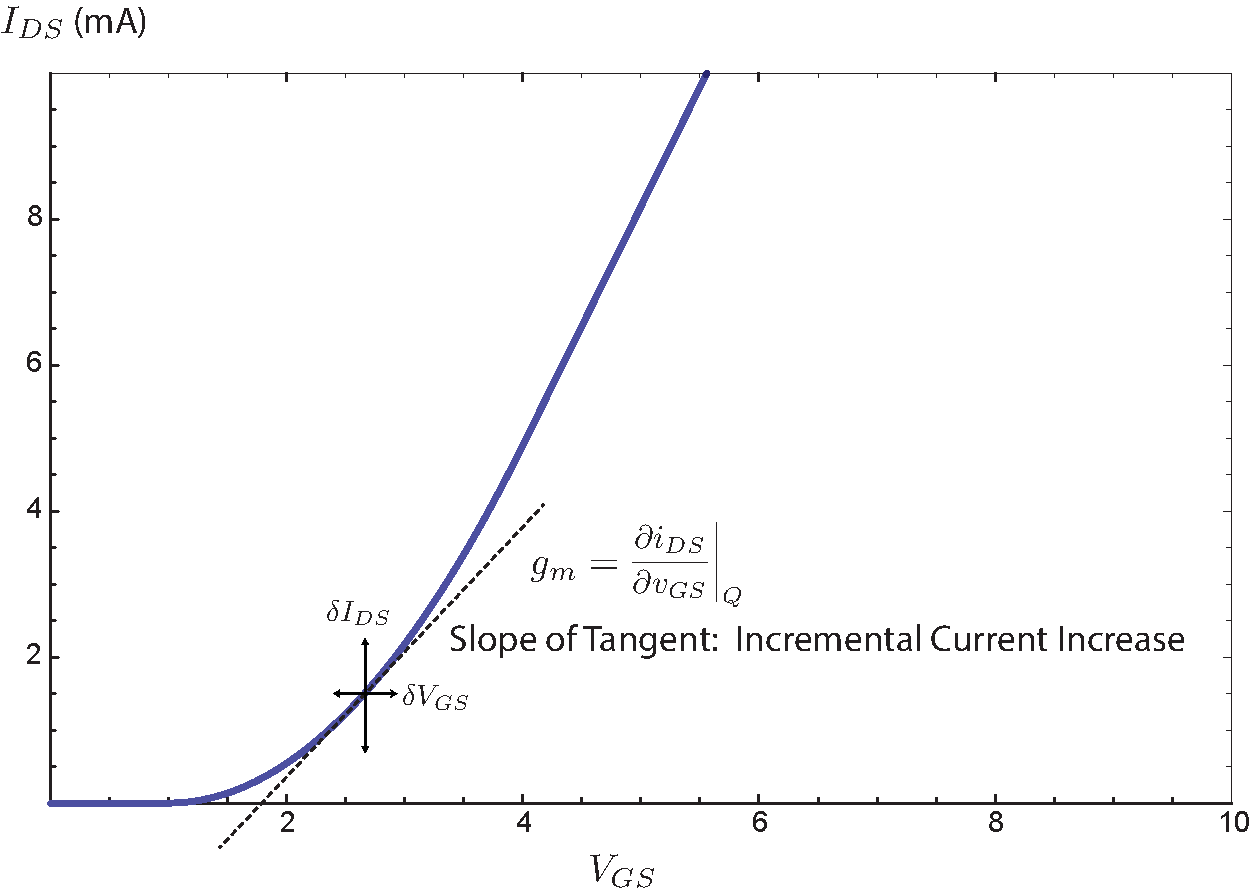
\includegraphics[width=.75\columnwidth]{id_vgs_slope}
\caption{The transconductance $g_m$ is the slope of the $I_{DS}$ vs $V_{GS}$ curve for a fixed value of $V_{DS}$.}
\label{fig:id_vgs_slope}
\end{figure}
%%%%%%%%%%%%%%%%%%%%%%%%%%%%%%%%%%%%%%%%%%%%
%             SUBSECTION 9.4.2             %
%%%%%%%%%%%%%%%%%%%%%%%%%%%%%%%%%%%%%%%%%%%%
\subsection{The MOS \textit{Transconductance}}
In saturation the drain-source current is given by:
    \begin{equation}
        {I_{DS,sat}} = \frac{W}{L}\frac{{\mu {C_{ox}}}}{2}{({V_{GS}} - {V_T})^2}(1 + \lambda {V_{DS}})
        \label{eq:ids}
    \end{equation} 
By using the definition of transconductance, the change in drain current due to a change in the \textit{gate-source} voltage, with \textit{everything else constant}, we evaluate the derivative of $I_{DS,sat}$ with respect to $V_{GS}$:
    \begin{equation}
        {g_m} = {\left. {\frac{{\Delta {i_D}}}{{\Delta {v_{GS}}}}} \right|_{{V_{GS,}}{V_{DS}}}} = {\left. {\frac{{\partial {i_D}}}{{\partial {v_{GS}}}}} \right|_{{V_{GS,}}{V_{DS}}}} = \mu {C_{ox}}\frac{W}{L}({V_{GS}} - {V_T})(1 +\underbrace{ \lambda {V_{DS}}}_{\approx 0})
    \end{equation}
    \begin{equation}
        {g_m} = \mu {C_{ox}}\frac{W}{L}({V_{GS,Q}} - {V_T}) = \mu {C_{ox}}\frac{W}{L}(V_{DS,sat})
    \end{equation}
This equation shows that $g_m$ is a strong function of the gate-overdrive voltage, defined as the gate bias beyond threshold, $V_{GS} - V_T$, and the device mobility $\mu$ and gate-oxide capacitance $C_{ox}$.  We can write $g_m$ in other equivalent forms, for instance by substitution of $V_{GS}-V_T$ from \emph{Eq.~\ref{eq:ids}} (with $\lambda = 0$):
    \begin{equation}
        {g_m} = \mu {C_{ox}}\frac{W}{L}\sqrt {\frac{{2{I_{DS}}}}{{\frac{W}{L}\mu {C_{ox}}}}}  = \sqrt {2\mu{C_{ox}}\frac{W}{L}{I_{DS}}}
    \end{equation}
which shows the $g_m$ increases like $\sqrt{I_{DS}}$ with increasing bias.  Finally, we can express $g_m$ in a third way by dividing \emph{Eq.~\ref{eq:ids}} by $V_{GS}-V_T$:
    \begin{equation}
        {g_m} = \frac{{2{I_{DS}}}}{{({V_{GS}} - {V_T})}} \label{eq:gm_vstar}
    \end{equation} 
This form may seem the most ambiguous, because it depends on both the bias current and the gate-overdrive, but it turns out to be a very useful way to compare the required $g_m$ to meet certain specifications, as we will show in the following chapters.
%%%%%%%%%%%%%%%%%%%%%%%%%%%%%%%%%%%%%%%%%%%%
%             SUBSECTION 9.4.3             %
%%%%%%%%%%%%%%%%%%%%%%%%%%%%%%%%%%%%%%%%%%%%
\subsection{Output Resistance \texorpdfstring{$r_o$}{}}
%%%%%%%%%%%%%%%%%%%%%%%%%%%%%%%%%%%%%%%%%%%%
%                 FIGURE                   %
%%%%%%%%%%%%%%%%%%%%%%%%%%%%%%%%%%%%%%%%%%%%
\begin{figure}[tb]
\centering
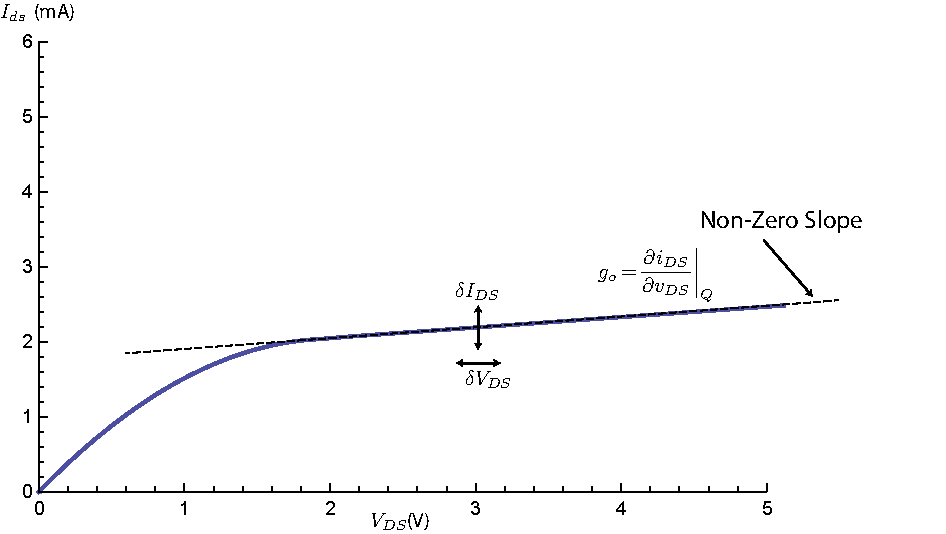
\includegraphics[width=.75\columnwidth]{ids_idsat_ro}
\caption{The output conductance $g_o$ is the slope of the $I_{DS}$ vs $V_{DS}$ curve for a fixed value of $V_{GS}$.  It's more common to state the output resistance $r_o = g_o^{-1}$.}
\label{fig:ids_idsat_ro}
\end{figure}
%%%%%%%%%%%%%%%%%%%%%%%%%%%%%%%%%%%%%%%%%%%%
We again start with \emph{Eq.~\ref{eq:ids}}, but now to find $g_o$ ($1/r_o$), defined as the change in drain current due to a change in the \textit{drain-source} voltage, with \textit{everything else constant}.  In other words:
    \begin{equation}
        {g_o} = \,{ {{{\left. {\frac{{\partial {i_D}}}{{\partial {v_{DS}}}}} \right|}_{{V_{GS}},{V_{DS}}}}} }
    \end{equation}
or
    \begin{equation}
        {r_o} = \,{\left( {{{\left. {\frac{{\partial {i_D}}}{{\partial {v_{DS}}}}} \right|}_{{V_{GS}},{V_{DS}}}}} \right)^{ - 1}}
    \end{equation}
Since the current in \emph{Eq.~\ref{eq:ids}} is only a linear function of $V_{DS}$, the derivative is easy to evaluate:
    \begin{equation}
        {r_o} = \frac{1}{{\frac{W}{L}\frac{{\mu {C_{ox}}}}{2}{{({V_{GS}} - {V_T})}^2}\lambda }}
    \end{equation}
If $\lambda$ is small, then the current is approximately the term in the denominator:
    \begin{equation}
        {r_o} \approx \frac{1}{{\lambda {I_{DS}}}}
    \end{equation}
%%%%%%%%%%%%%%%%%%%%%%%%%%%%%%%%%%%%%%%%%%%%
%             SUBSECTION 9.4.4             %
%%%%%%%%%%%%%%%%%%%%%%%%%%%%%%%%%%%%%%%%%%%%
\subsection{Small-Signal Model for MOSFET}
%%%%%%%%%%%%%%%%%%%%%%%%%%%%%%%%%%%%%%%%%%%%
%                 FIGURE                   %
%%%%%%%%%%%%%%%%%%%%%%%%%%%%%%%%%%%%%%%%%%%%
\begin{figure}[tb]
\centering
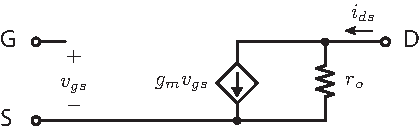
\includegraphics[scale=1]{mos3term_ac_nocap}
\caption{The small-signal equivalent circuit model of a NMOS device.  This is a three terminal model and does not include any charge storage effects.}
\label{fig:mos3term_ac_nocap}
\end{figure}
%%%%%%%%%%%%%%%%%%%%%%%%%%%%%%%%%%%%%%%%%%%%
If we translate the derived equation for the small-signal linearized current, repeated here for convenience,
    \begin{equation}
        {i_{ds}} = {g_m}{v_{gs}} + \frac{1}{{{r_o}}}{v_{ds}}
    \end{equation}
into a circuit diagram, we obtain the simplified  3-terminal small-signal model for a MOSFET shown in \emph{Fig.~\ref{fig:mos3term_ac_nocap}}.  In the next chapter, we will develop a more complete model.  It's important to note that once you specify the DC operating point of an amplifier, you also fix the small-signal parameters.  Thus to determine the small-signal circuit, you only need to know the DC operating point.
%%%%%%%%%%%%%%%%%%%%%%%%%%%%%%%%%%%%%%%%%%%%
%             SUBSECTION 9.4.5             %
%%%%%%%%%%%%%%%%%%%%%%%%%%%%%%%%%%%%%%%%%%%%
\subsection{Small-Signal Analysis Steps:  The "Easy Way"}
Earlier we solved for the small-signal response of the amplifier the "hard way".  Now we have introduced a systematic approach.  We can summarize the small-signal analysis technique by breaking it down into simple steps:
    \begin{enumerate}
    	\item  Calculate bias points using DC sources
    	\item  Use the bias point to determine the MOSFET region of operation as well as to calculate small-signal parameters
    	\item  Turn off DC sources in the schematic (short DC voltages, open DC currents)
    	\item  Redraw the schematic by using the small-signal model for the MOSFET in place of the transistor
    	\item  Calculate the gain ($v_{out}/v_{in}$) of the circuit, or any other parameter of interest.
    \end{enumerate}
%%%%%%%%%%%%%%%%%%%%%%%%%%%%%%%%%%%%%%%%%%%%
%              SUB-SUBSECTION              %
%%%%%%%%%%%%%%%%%%%%%%%%%%%%%%%%%%%%%%%%%%%%
\subsubsection{Small Signal Analysis:  Step 1 and 2}
We already found the DC operating point in the earlier part of this chapter.  From the DC operating point we can next calculate the small-signal parameters of the transistor:
    \begin{equation}
        {g_m} = \frac{{2{I_{DS}}}}{{({V_{GS}} - {V_T})}}
    \end{equation}
    \begin{equation}
        {r_o} \approx \frac{1}{{\lambda {I_{DS}}}}
    \end{equation}
%%%%%%%%%%%%%%%%%%%%%%%%%%%%%%%%%%%%%%%%%%%%
%              SUB-SUBSECTION              %
%%%%%%%%%%%%%%%%%%%%%%%%%%%%%%%%%%%%%%%%%%%%
\subsubsection{Small Signal Analysis:  Step 3}
%%%%%%%%%%%%%%%%%%%%%%%%%%%%%%%%%%%%%%%%%%%%
%                 FIGURE                   %
%%%%%%%%%%%%%%%%%%%%%%%%%%%%%%%%%%%%%%%%%%%%
\begin{figure}[tb]
\centering
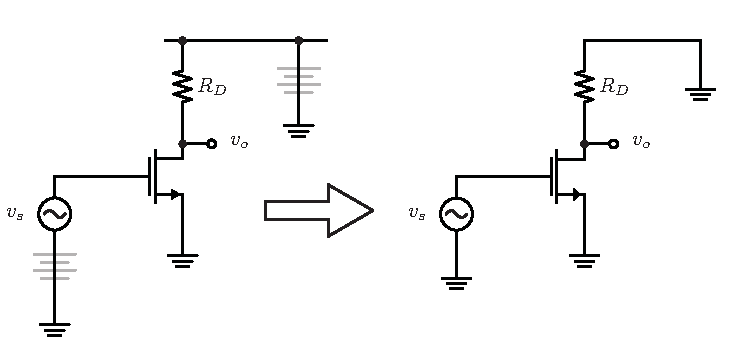
\includegraphics[scale=1]{cs_amp_ac}
\caption{The AC model of a the amplifier is produced by shorting out all DC voltage sources.} \label{fig:cs_amp_ac}
\end{figure}
%%%%%%%%%%%%%%%%%%%%%%%%%%%%%%%%%%%%%%%%%%%%
In this step we turn off all DC sources, as shown in \emph{Fig.~\ref{fig:cs_amp_ac}}.  The DC voltage sources become shorts and DC current sources become opens.
%%%%%%%%%%%%%%%%%%%%%%%%%%%%%%%%%%%%%%%%%%%%
%              SUB-SUBSECTION              %
%%%%%%%%%%%%%%%%%%%%%%%%%%%%%%%%%%%%%%%%%%%%
\subsubsection{Small Signal Analysis:  Step 4}
%%%%%%%%%%%%%%%%%%%%%%%%%%%%%%%%%%%%%%%%%%%%
%                 FIGURE                   %
%%%%%%%%%%%%%%%%%%%%%%%%%%%%%%%%%%%%%%%%%%%%
\begin{figure}[tb]
\centering
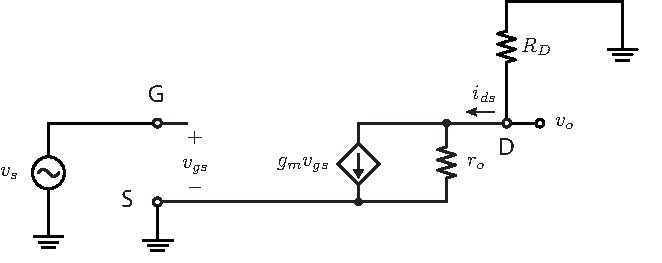
\includegraphics[scale=1]{cs_amp_ss1}
\caption{The small-signal AC model of the NMOS CS amplifier. Note that this is derived by replacing the NMOS transistor (\emph{Fig.~\ref{fig:cs_amp_ac}}) with its small-signal equivalent circuit (\emph{Fig.~\ref{fig:mos3term_ac_nocap}}).}
\label{fig:cs_amp_ss1}
\end{figure}
%%%%%%%%%%%%%%%%%%%%%%%%%%%%%%%%%%%%%%%%%%%%
Now we draw a new schematic, by replacing the transistor with its small-signal model, shown in \emph{Fig.~\ref{fig:cs_amp_ss1}}.  As you become more proficient at analyzing transistor circuits, you can sometimes avoid this step. But that'll come later, maybe in this class or maybe in your next.  For now it's totally okay to just draw out the circuit to familiarize yourself with it.
%%%%%%%%%%%%%%%%%%%%%%%%%%%%%%%%%%%%%%%%%%%%
Instead of a "macro" replacement, you should actually redraw the circuit to simplify the connections and make things as obvious as possible. This will facilitate "inspection" style analysis. For example, you'll be able to identify that $R_D$ and $r_o$ are in parallel, so you can treat them as a single equivalent resistor.  See \emph{Fig.~\ref{fig:cs_amp_ss2}}.
%%%%%%%%%%%%%%%%%%%%%%%%%%%%%%%%%%%%%%%%%%%%
%                 FIGURE                   %
%%%%%%%%%%%%%%%%%%%%%%%%%%%%%%%%%%%%%%%%%%%%
\begin{figure}[tb]
\centering
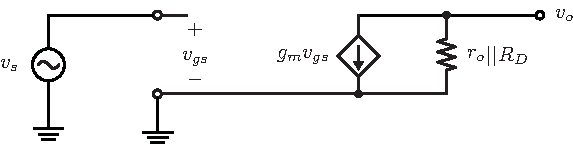
\includegraphics[scale=1]{cs_amp_ss2}
\caption{A simplified small-signal AC model of the amplifier, derived from \emph{Fig.~\ref{fig:cs_amp_ss1}}.} \label{fig:cs_amp_ss2}
\end{figure}
%%%%%%%%%%%%%%%%%%%%%%%%%%%%%%%%%%%%%%%%%%%%
%              SUB-SUBSECTION              %
%%%%%%%%%%%%%%%%%%%%%%%%%%%%%%%%%%%%%%%%%%%%
\subsubsection{Small Signal Analysis:  Step 5}
Now we are ready to analyze the circuit like any other linear AC circuit.  You can find the gain, the input/output impedance, etc.  This circuit is very easy to analyze, and the output voltage is given by
    \begin{equation}
        v_o = -g_m v_{gs} \cdot r_o || R_D 
    \end{equation}
Notice that the input signal $v_s$ is actually the same as $v_{gs}$, so we have
    \begin{equation}
        A_v = \frac{v_o}{v_s} = -g_m r_o || R_D
    \end{equation}
We have the device output resistance in this analysis "for free" where we neglected it in the "hard way" analysis we did earlier.   Still the final answer doesn't seem to agree with our earlier analysis.  To see why, first write $g_m$ in terms of the transistor bias.  In this case, it's convenient to use this form
    \begin{equation}
        g_m = \frac{2 I_{DS,Q}}{V_{GS,Q}-V_T}
    \end{equation}
    \begin{equation}
        A_v =  -\frac{2 I_{DS} r_o||R_D}{V_{GS}-V_T}
    \end{equation}
If we assume $r_o \gg R_D$, then we get the same result as before because $I_D R_D = \frac{V_{DD}}{2}$:
    \begin{equation}
        A_v \approx  -\frac{2 I_{DS} R_D}{V_{GS}-V_T} = \frac{2\frac{V_{DD}}{2} }{V_{GS}-V_T} = \frac{V_{DD}}{V_{GS}-V_T}
    \end{equation}
%%%%%%%%%%%%%%%%%%%%%%%%%%%%%%%%%%%%%%%%%%%%%%%%%%%%%%%%%%%%%%%%%%%%%%%%%%%%%%%%%%%%%%%%
%%%%%%%%%%%%%%%%%%%%%%%%%%%%%%%%%%%%%%%%%%%%%%%%%%%%%%%%%%%%%%%%%%%%%%%%%%%%%%%%%%%%%%%%
%                                   SECTION 9.5                                        %
%%%%%%%%%%%%%%%%%%%%%%%%%%%%%%%%%%%%%%%%%%%%%%%%%%%%%%%%%%%%%%%%%%%%%%%%%%%%%%%%%%%%%%%%
%%%%%%%%%%%%%%%%%%%%%%%%%%%%%%%%%%%%%%%%%%%%%%%%%%%%%%%%%%%%%%%%%%%%%%%%%%%%%%%%%%%%%%%%
\section{PMOS Amplifier and Small-Signal Model}
%%%%%%%%%%%%%%%%%%%%%%%%%%%%%%%%%%%%%%%%%%%%
%             SUBSECTION 9.5.1             %
%%%%%%%%%%%%%%%%%%%%%%%%%%%%%%%%%%%%%%%%%%%%
\subsection{Small-Signal PMOS Model}
%%%%%%%%%%%%%%%%%%%%%%%%%%%%%%%%%%%%%%%%%%%%
%                 FIGURE                   %
%%%%%%%%%%%%%%%%%%%%%%%%%%%%%%%%%%%%%%%%%%%%
\begin{figure}[tb]
\centering
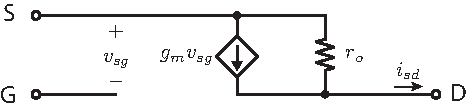
\includegraphics[scale=1]{pmos3term_dc}
\caption{The PMOS small-signal equivalent circuit model.  Compare with \emph{Fig.~\ref{fig:mos3term_ac_nocap}}.}
\label{fig:pmos3term_dc}
\end{figure}
%%%%%%%%%%%%%%%%%%%%%%%%%%%%%%%%%%%%%%%%%%%%
So far we have focused on the NMOS device. Let's introduce the PMOS small-signal model shown in \emph{Fig.~\ref{fig:pmos3term_dc}}.  This model looks like an upside down NMOS model.  Remember that the current flows from the source to the drain of a PMOS (from higher potential to lower potential).  In an NMOS, the drain is at a higher potential, so you must flip the model around.   A good way to sanity check is to "wiggle" the gate of the transistor and observe what the model predicts and make sure the polarity is correct.  If we increase the gate voltage for a PMOS, we're reducing the inversion layer conductance, so the current should go down. Note that the small-signal model agrees and shows the current going negative.
%%%%%%%%%%%%%%%%%%%%%%%%%%%%%%%%%%%%%%%%%%%%
%             SUBSECTION 9.5.2             %
%%%%%%%%%%%%%%%%%%%%%%%%%%%%%%%%%%%%%%%%%%%%
\subsection{PMOS Amplifier}
%%%%%%%%%%%%%%%%%%%%%%%%%%%%%%%%%%%%%%%%%%%%
%                 FIGURE                   %
%%%%%%%%%%%%%%%%%%%%%%%%%%%%%%%%%%%%%%%%%%%%
\begin{figure}[tb]
\begin{center}
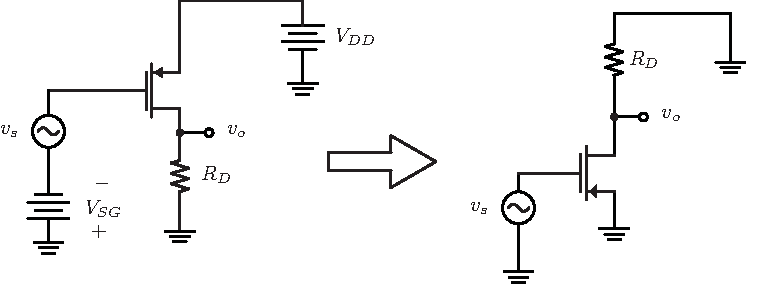
\includegraphics[scale=1]{cs_amp_pmos_ss1}
\end{center}
\caption{The PMOS CS amplifier and its AC equivalent circuit.}
\label{fig:cs_amp_pmos_ss1}
\end{figure}
%%%%%%%%%%%%%%%%%%%%%%%%%%%%%%%%%%%%%%%%%%%%
We take the same exact steps as in the NMOS amplifier to produce an amplifier with a PMOS device, shown in \emph{Fig.~\ref{fig:cs_amp_pmos_ss1}}.  Note this is a "Common Source" Amplifier even though the PMOS source connects to DC supply.  \textbf{DC supplies are AC grounds, so the source is actually AC grounded.}   The small-signal model of the amplifier is drawn in \emph{Fig.~\ref{fig:csamp_pmos_ss}}, and it is identical to the NMOS case.  So there's no reason to redo the math.
%%%%%%%%%%%%%%%%%%%%%%%%%%%%%%%%%%%%%%%%%%%%
Which is better, the NMOS or PMOS?  Traditionally NMOS amplifiers are preferred because the electron mobility is higher, leading to higher $g_m$ and thus higher gain.  But PMOS amplifiers are also useful and will be used extensively.  Namely when you need to "flip" the DC bias around, you can use an cascade of an NMOS and PMOS and avoid large coupling capacitors.  That's jumping ahead but you'll see NMOS and PMOS amplifiers used together in cascade often by the end of this book.  
%%%%%%%%%%%%%%%%%%%%%%%%%%%%%%%%%%%%%%%%%%%%
%                 FIGURE                   %
%%%%%%%%%%%%%%%%%%%%%%%%%%%%%%%%%%%%%%%%%%%%
\begin{figure}[tb]
\centering
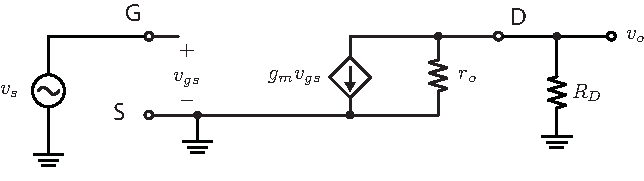
\includegraphics[scale=1]{csamp_pmos_ss}
\caption{The re-drawn PMOS small-signal AC schematic, which is identical to the NMOS case.} \label{fig:csamp_pmos_ss}
\end{figure}
%%%%%%%%%%%%%%%%%%%%%%%%%%%%%%%%%%%%%%%%%%%%%%%%%%%%%%%%%%%%%%%%%%%%%%%%%%%%%%%%%%%%%%%%
%%%%%%%%%%%%%%%%%%%%%%%%%%%%%%%%%%%%%%%%%%%%%%%%%%%%%%%%%%%%%%%%%%%%%%%%%%%%%%%%%%%%%%%%
%                                   SECTION 9.6                                        %
%%%%%%%%%%%%%%%%%%%%%%%%%%%%%%%%%%%%%%%%%%%%%%%%%%%%%%%%%%%%%%%%%%%%%%%%%%%%%%%%%%%%%%%%
%%%%%%%%%%%%%%%%%%%%%%%%%%%%%%%%%%%%%%%%%%%%%%%%%%%%%%%%%%%%%%%%%%%%%%%%%%%%%%%%%%%%%%%%
\section{What We've Ignored}
We have actually made a lot of approximations up to now.  But simplicity is a good thing and the models we developed in this chapter will form the core of our analysis and intuition.  When we want to model other "second-order" effects, we must in some cases introduce the fourth terminal of the MOSFET, or bring back the body of the transistor.  We'll show that the body of the transistor acts like a second gate, or "back gate", and cannot be ignored if the body-source voltage is moving around.  We also know that the source/drain junctions of the transistor form $PN$-junction diodes with body, which  introduces parasitic capacitance.  In fact, we also ignored the gate-oxide capacitance. It turns out that we can simply add many of these capacitors to our small-signal model, as we'll show in the next chapter.
%%%%%%%%%%%%%%%%%%%%%%%%%%%%%%%%%%%%%%%%%%%%
Also modern transistors are very short channel length devices, and there are many "short channel" effects that we're ignoring, such as velocity saturation and other "high field" effects.  Finally we have been assuming that you have to bias the transistor in the strong inversion region $V_{GS} > V_T$, but it turns out that even with moderate inversion, or even sub-threshold bias, the transistor still behaves like a transistor for AC signals.  This is especially useful in low power circuits which are preferentially biased in moderate or weak-inversion (sub-threshold).  This is a more advanced topic that you can learn in your next course on circuit design.
